
\setcounter{section}{0}

\setcounter{figure}{0}
\setcounter{table}{0}
\setcounter{equation}{0}
%==========================================



\chapter{双电子谱测量}

%!TEX encoding = UTF-8 Unicode
正如绪论当中提到的,双轻子是一个研究相对论重离子对撞的一个很好的物理探针。STAR前期的双电子谱测量当中,受限于统计和以及高对撞能量下较高的来源于重味夸克半轻子衰变的原因,在中等质量区间内抽取来源于夸克胶子等离子体热辐射的产额变得十分困难。STAR在2017年采集了有着高统计量的 \sNN = 54.4 GeV金-金对撞的数据。其既有较高的统计量,又相对于\sNN = 200 GeV 在中等质量区间有着较低的重味夸克半轻子衰变的产额,是一个在RHIC能区下测量中等质量区间双轻子额外产额的好机会。

\section{数据集和事例判选}
STAR于2017年采集了质心系能量为54.4GeV最小无偏(Minimum bias, MB)金-金对撞的数据。在此数据集中,中心度(Centrality)的定义由Glauber模型计算得到的带电粒子多重数得出。  通过将中间快度区域($|\eta| < 0.5 $)的带电粒子多重数分布均分得到每个中心度对应的带电粒子多重数区间。表 \ref{tab:centrality} 列举出了54.4 GeV 金-金对撞中不同中心度区间对应的带电粒子多重数(RefMult)范围。由于探测器触发(Triggeer)效率的影响,当发生偏心碰撞时实际探测到的带电粒子多重数分布和理论计算存在差异,所以一个权重修正被引入来修正实际数据和理论计算的差距。修正后的带电粒子多重数(RefMultCorr)用来进行最终的中心度计算。本分析中所分析的数据中心度区间为0-80\%。

\begin{table}[h!]
    \centering
    \caption{不同中心度带电粒子多重数范围}
    \label{tab:centrality}
    \begin{tabular}{|c|c|}
    \hline
        中心度 & 带电粒子多重数最小值  \\
    \hline
         0-5\% & 361  \\
     \hline
         5-10\% & 299  \\
    \hline
         10-20\% & 205  \\
    \hline
         20-30\% & 138  \\
    \hline
         30-40\% & 89  \\
    \hline
         40-50\% & 54  \\
    \hline
         50-60\% & 31  \\
    \hline
         60-70\% & 16  \\
    \hline
         70-80\% & 7   \\     
    \hline
    \end{tabular}
\end{table}

为了提高分析中所用到的事例(Event)质量,几个关于事例质量的判选条件被添加到了分析中。如表 \ref{tab:EventSelection} 所示。通过事例质量筛选后所剩事例数约为800M

\begin{table}[h!]
    \centering
    \caption{事例判选条件}
    \label{tab:EventSelection}
    % \begin{tabularx}{0.8\textwidth} {
    % | >{\centering\arraybackslash}X | >{\centering\arraybackslash}X | }
    \begin{tabular}{|c|c|}
        \hline
        Trigger ID & Minbias (580001,580021)  \\
        \hline
        Vertex & $|V_z| < 35cm ~\&\&~ V_r < 2cm$   \\
        \hline
        Vertex Difference & $|V_{z}^{TPC} - V_{z}^{VPD}| < 3cm$\\
        \hline
    \end{tabular}
\end{table}

\section{径迹判选和电子鉴别}
在每次54.4 GeV 金-金对撞当中,末态平均有几百条径迹被STAR探测器所探测到。为了从中挑选出合格的电子径迹用来进行最后的分析,一些关于径迹质量和粒子鉴别的判选条件被应用在了本分析当中。下面的章节将对这两组判选条件进行详细的介绍。
\subsection{径迹判选}
\label{chap:track_selection}
在本分析中,主要用到的子探测器是时间投影室和飞行时间探测器。由于探测器本身的限制,分析中所用到的径迹应该在这两个探测器的接收度范围内,且可以被探测器很好地重建出来。
这样一来,分析中所用到的进行电子对重建的电子的径迹应该满足探测器接收度和径迹重建质量上的需求,从而保证整个分析的质量。

对于一条满足径迹重建质量要求的径迹来说,其对应的粒子在穿越时间投影室的过程中应该留下了足够多的击中来进行径迹重建。自然在本分析当中就对径迹用来重建的击中数(nHitsFit)有了要求。当两条粒子的径迹在空间位置上很近的时候,这两个粒子在时间投影室中留下的击中就容易被算法认为属于同一个粒子留下的径迹中的击中。为了避免这种情况,一条径迹用来重建的击中数和最大可利用击中数的比值(nHitsfit/nHitsPoss)应该大于0.52。时间投影室是利用粒子穿过漂移区域时的电离能损信息来进行粒子鉴别的,其具体方法在\ref{chap:TPC}当中已进行过讨论。那么和重建类似,一条满足径迹重建质量要求的径迹也需要留下足够多的击中来进行能量损失的计算,这也就对径迹用来计算电离能损的击中数(nHitsDedx)有了要求。
在本分析当中所研究的电子对都来源于夸克胶子等离子体或者短寿命的介子衰变,这意味着电子应该来源于主碰撞顶点(Primary Vertex)而不是离主碰撞顶点较远的次级衰变顶点。为了满足这个要求,一个关于径迹到主碰撞顶点的最近距离(distance of closest approach,DCA)的盘旋条件被添加到了分析当中。

详细的径迹质量判选条件和径迹的接收度范围在表\ref{tab:TrackQuality}左栏中列出。

\begin{table}[h!]
    \centering
    \caption{径迹质量和电子鉴别(eID)判选条件}
    \label{tab:TrackQuality}
    \begin{tabularx}{0.8\textwidth} {
    | >{\centering\arraybackslash}X |>{\centering\arraybackslash}X | }
        \hline
        径迹质量判选 & 电子鉴别(eID)   \\
        \hline
        $0.2 \leq p_{T} \leq 30 GeV/c $ & $p<0.8 GeV/c $ \\
        $|\eta| \leq 1 $ & $ 3*p - 3.15 \leq |n\sigma_{e}| \geq 2.0$  \\
        $dca \leq 1cm $ & $p \geq 0.8 GeV/c $\\ 
        $N_{HitsFit} \geq 20 $  & $ -0.75 \leq |n\sigma_{e}| \geq 2.0 $\\
        ${N_{HitsFit}}/{N_{HitsPoss}} \geq 0.52 $ &  $|1-1/\beta| < 0.25 $\\
        $N_{HitsDedx} \geq 15 $  & \\
        \hline
    \end{tabularx}
\end{table}

\subsection{电子鉴别(eID)}
\label{ch:eID}
当选出了符合径迹重建质量要求的径迹之后,再通过径迹的电离能损和速度信息就可以辨别出来径迹有没有可能为一条由电子留下来的径迹。
将每条径迹由时间投影室测量得到的电离能损和通过Bethe-Bloch公式计算得到的电子电离能损相比较后再由探测器的分辨率进行归一化便可以得到一个用来表明径迹为电子径迹的可能性的一个值,\nSigmaE 。具体计算公式如式\ref{eq:nSigmaE}所示。在理想情况下,电子的$n\sigma_\mathrm{e}$应该为一个中心值为0宽度为1的高斯分布。在径迹的动量比较高的时候,电子在工作气体中的电离能损和其他粒子重合,无法单独通过电离能损鉴别粒子。这时可以通过结合电离能损和飞行时间探测器所测得的速度信息来进行粒子鉴别。因为电子质量轻于其它强子,在相同动量下电子的速度会大于其他强子。这就意味着可以额外添加一个$1/\beta$的判选条件来进行电子鉴别。电子鉴别的条件在表\ref{tab:TrackQuality}的右栏列出。图 \ref{beta_Cut}和\ref{fig:nSigmaEwTOF}分别为$1/\beta$的分布和加上$1/\beta$判选条件后的$n\sigma_\mathrm{e}$分布。

\begin{equation}
    \label{eq:nSigmaE}
    n\sigma_e = \frac{log(\frac{dE/dx_{measure}}{dE/dx_{BB}})}{\sigma_{dE/dx}}
\end{equation}

\begin{figure}[htb]
    \centering
    \begin{subfigure}[b]{0.45\textwidth}
        \centering
        \includegraphics[width=\textwidth,clip]{figures/Chapter4/nSigmaEwTOF.png}
        \caption{}
        \label{fig:nSigmaEwTOF}
    \end{subfigure}
    \hfill
    \begin{subfigure}[b]{0.49\textwidth}
        \centering
        \includegraphics[width=\textwidth,clip]{figures/Chapter4/beta_Cut.png}
        \caption{}
        \label{fig:beta_Cut}
    \end{subfigure}
       \caption[\nSigmaE 和 $1/\beta$判选条件示意图]{图\ref{fig:nSigmaEwTOF}为\nSigmaE 判选条件示意图,其中黑色虚线为\sNN = 54.4GeV 中 \nSigmaE 的判选条件上下限。图 \ref{fig:beta_Cut}为$1/\beta$判选条件示意图, 黑色实线为判选条件上下限 }
       \label{fig:eID_cut}
\end{figure}

\subsection{电子样本纯度}
\label{chap:pruity}

从图\ref{fig:nSigmaEwTOF}可以看到,尽管通过\nSigmaE 和$1/\beta$的判选条件可以有效的选出电子样本,但仍然有一部分强子的\nSigmaE 分布会和电子的有所覆盖。这样就需要估计强子在电子样本当中所占的比重,即强子污染(hadron contamination)。

为了估计强子污染,首先要得到纯的强子以及电子样本的\nSigmaE 分布。这就需要通过某种方法挑选出纯强子和纯电子的数据样本,在本分析中纯强子样本是通过添加一个严苛的质量判选条件和比较宽松的$n\sigma_{hadron}$判选条件的方法挑选得到的。对于不同的强子,其质量判选条件在表\ref{tab:pure_sample}当中列出。当两条径迹的电荷相同、动量相似的时候,这两条径迹在时间投影室当中留下的击中会非常接近,这就使得这两条径迹在重建的时候很容易被重建成一条径迹,这就是merged track。在金-金对撞当中,因为末态大多数的带电粒子为$\pi$介子,所以我们在选取纯强子样本的时候把merged $\pi$也一并考虑了进来。
图\ref{fig:pure_hadron_sample}中为纯$\rm{\pi/k/p}$样本以及 merged $\pi$ 样本的$\rm{n\sigma_{e}~v.s.~p}$的二维分布。

\begin{table}[]
    \centering
    \caption{选取纯$\rm{\pi/k/p}$样本时的质量判选条件}
    \begin{tabular}{|c|c|}
        \hline
        particle & mass cut  \\
        \hline
        $\pi$ & $ 0.019 \pm 0.003 GeV/c^2$\\
        \hline
        $Kaon$ & $ 0.243 \pm 0.005 GeV/c^2$\\
        \hline
        $Proton$ & $ 0.879 \pm 0.020 GeV/c^2$ \\
        \hline
    \end{tabular}
    \label{tab:pure_sample}
\end{table}

\begin{figure}[h!]
    \centering
    \begin{subfigure}[h!]{0.43\textwidth}
            \includegraphics[width=\textwidth]{figures/Chapter4/PurePion.png}
            \caption{}
            \label{fig:PurePion}
    \end{subfigure}
    \begin{subfigure}[h!]{0.43\textwidth}
            \includegraphics[width=\textwidth]{figures/Chapter4/PureKaon.png}
            \caption{}
            \label{fig:PureKaon}
    \end{subfigure}

    \begin{subfigure}[h!]{0.43\textwidth}
            \includegraphics[width=\textwidth]{figures/Chapter4/PureProton.png}
            \caption{}
            \label{fig:PureProton}
    \end{subfigure}
    \begin{subfigure}[h!]{0.43\textwidth}
            \includegraphics[width=\textwidth]{figures/Chapter4/PureMergePion.png}
            \caption{}
            \label{fig:PureMergePion}
    \end{subfigure}
    \caption[纯$\rm{\pi/k/p}$样本以及 merged $\pi$ 样本的$\rm{n\sigma_{e}~v.s.~p}$的二维分布]{纯$\rm{\pi/k/p}$样本以及 merged $\pi$ 的  $\rm{n\sigma_{e}~v.s.~p}$的二维分布。左上:$\pi$介子;右上:K介子;左下:质子;右下:merged $\pi$ }
    \label{fig:pure_hadron_sample}
\end{figure}

而纯电子样本是通过挑选来自于$\pi^0$的Dalitz衰变以及光子转换的电子对得到的。如\ref{chap:photon_conversion}小节当中所讨论的一样,光子击中探测器材料所产生的正负电子对其质量应该为0,但因为primary track要求通过碰撞顶点的原因导致其重建出来之后有一个很小的不变质量。这样如果选取不变质量很小的双电子对来选取纯电子数据样本。
在本分析中所用到的挑选纯电子数据样本的判选条件为$\rm{M_{ee} < 0.015~GeV/c^2}$,如图\ref{fig:PureElectron_cut}所示。在图中可以看到在这个质量区间内双电子信号的信噪比很高,在0-80\%中心度下可以达到129.97的信噪比,纯电子数据样本的$n\sigma_e$分布如图\ref{fig:PureElectron_Sample}所示。

\begin{figure}[h!]
    \centering
    \begin{subfigure}[h!]{0.45\textwidth}
            \includegraphics[width=\textwidth]{figures/Chapter4/PureElectron_cut.png}
            \caption{}
            \label{fig:PureElectron_cut}
    \end{subfigure}
    \begin{subfigure}[h!]{0.45\textwidth}
            \includegraphics[width=\textwidth]{figures/Chapter4/PureElectron_Sample.png}
            \caption{}
            \label{fig:PureElectron_Sample}
    \end{subfigure}
    \caption[纯电子数据样本选取的判选条件以及纯电子样本的$\rm{n\sigma_{e}~v.s.~p}$的二维分布]{纯电子数据样本选取的判选条件(左图)以及纯电子样本的$\rm{n\sigma_{e}~v.s.~p}$的二维分布(右图)}
    \label{fig:PureElectron_sample_total}
\end{figure}

在得到纯强子以及纯电子数据样本之后,就可以在不同的动量区间内通过拟合的方式得到各个粒子样本在不同区间内$n\sigma_{e}$分布的中心值和宽度。结果如图\ref{fig:MeanAndSigma_puresample}所示。基于这些结果,可以通过对总的数据样本进行多高斯拟合的方式来确定不同动量区间内的电子纯度。

\begin{figure}[h!]
    \centering
    \begin{subfigure}[h!]{0.45\textwidth}
            \includegraphics[width=\textwidth]{figures/Chapter4/Mean_pureSample.png}
            \caption{}
            \label{fig:Mean_pureSample}
    \end{subfigure}
    \begin{subfigure}[h!]{0.45\textwidth}
            \includegraphics[width=\textwidth]{figures/Chapter4/Sigma_PureSample.png}
            \caption{}
            \label{fig:Sigma_PureSample}
    \end{subfigure}
    \caption[不同粒子样本在不同动量区间内的$n\sigma_{e}$分布中心值以及宽度示意图]{不同粒子样本在不同动量区间内的$n\sigma_{e}$分布中心值(左图)以及宽度(右图)示意图}
    \label{fig:MeanAndSigma_puresample}
\end{figure}

从\label{fig:Mean_pureSample}可以看出,强子样本的$n\sigma_{e}$分布的中心值和电子样本的$n\sigma_{e}$分布中心值仍然有重叠的区间,这就导致
在进行多高斯拟合时,其单个高斯分布的产额在中心值重叠的区间会变得不稳定。以图\ref{fig:MultGaus_CorssOver_Region}中的分布为例,在这个动量区间内质子和电子的分布中心值以及宽度基本重合,这就导致二者的产额在实际拟合过程中可以被相对随机地分配。为了避免这样的问题发生,对总体数据进行了两轮的多高斯拟合,通过第一轮拟合来估计强子在不同区间内的产额,从而保证粒子的产额在拟合过程中保持稳定。
\begin{figure}[h!]
    \centering
    \begin{subfigure}[h!]{0.45\textwidth}
            \includegraphics[width=\textwidth]{figures/Chapter4/MultGaus_good.png}
            \caption{}
            \label{fig:MultGaus_good}
    \end{subfigure}
    \begin{subfigure}[h!]{0.45\textwidth}
            \includegraphics[width=\textwidth]{figures/Chapter4/MultGaus_CorssOver_Region.png}
            \caption{}
            \label{fig:MultGaus_CorssOver_Region}
    \end{subfigure}
    \caption[计算电子纯度的多高斯拟合在不同动量区间内拟合结果示意图]{计算电子纯度的多高斯拟合在不同动量区间内拟合结果示意图 左图质量区间: $ 0.72~<~p~<~0.76~GeV$.右图质量区间: $ 0.96~<~p~<~1.00~GeV$,其中右图的质量区间位于强子样本的$n\sigma_{e}$分布的中心值和电子样本的$n\sigma_{e}$分布有重叠的区间内}
    \label{fig:Multi-Gaussian}
\end{figure}

首先进行第一轮多高斯拟合,在这一轮拟合当中不同粒子的$n\sigma_{e}$高斯分布的中心值和宽度被固定为图\ref{fig:MeanAndSigma_puresample}中所示的值,仅有产额作为自由参数参与拟合。第一轮多高斯拟合结束之后可以得到各个粒子的产额随着动量变化的分布。如图\ref{fig:Fit_Interpolate_ConstValue_FirstRound}所示。可以看到,在$n\sigma_{e}$中心值有重叠的动量区间,产额拟合结果变得很不稳定。为了改进拟合的结果,在这些$n\sigma_{e}$分布有重叠的动量区间内对强子的产额进行指数拟合。在第二轮拟合当中,这些通过指数拟合得到的强子产额被设置为多高斯拟合时每个强子分量的产额参数并且固定,此时只有电子的产额会作为自由参数进行拟合,拟合结果如图\ref{fig:Fit_Interpolate_ConstValue}所示。
\begin{figure}[h!]
    \centering
    \begin{subfigure}[h!]{0.43\textwidth}
            \includegraphics[width=\textwidth]{figures/Chapter4/Fit_Interpolate_ConstValue_FirstRound.pdf}
            \caption{}
            \label{fig:Fit_Interpolate_ConstValue_FirstRound}
    \end{subfigure}
    \begin{subfigure}[h!]{0.43\textwidth}
            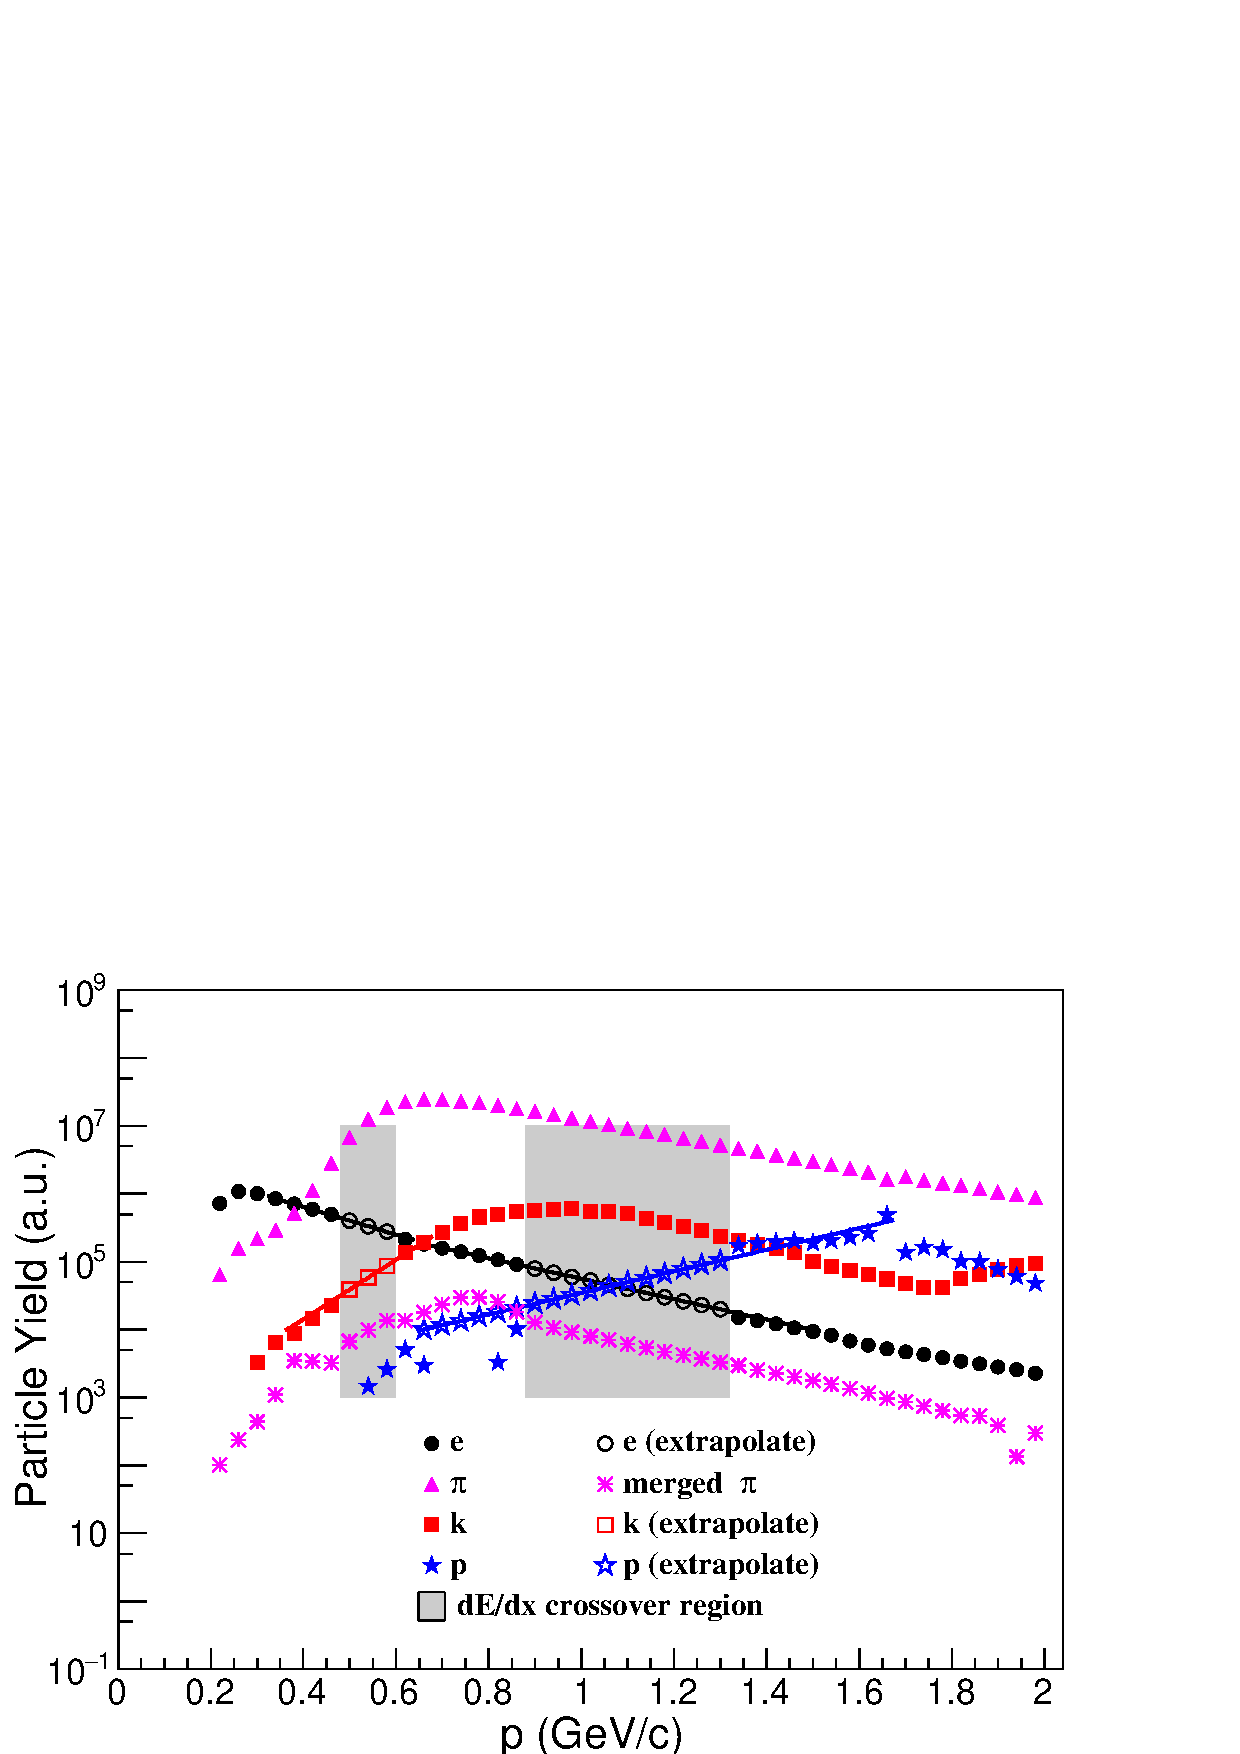
\includegraphics[width=\textwidth]{figures/Chapter4/Fit_Interpolate_ConstValue.pdf}
            \caption{}
            \label{fig:Fit_Interpolate_ConstValue}
    \end{subfigure}
    \caption[计算电子纯度时两轮高斯拟合的结果示意图]{计算电子纯度时两轮高斯拟合的结果示意图。左图为第一轮高斯拟合的结果,右图为第二轮高斯拟合的结果。灰色条带标出的区域为强子样本的$n\sigma_{e}$分布的中心值和电子样本的$n\sigma_{e}$分布有重叠的区间}
    \label{fig:Multi-Gaussian_result}
\end{figure}

在进行第二轮拟合的同时我们可以计算得到电子在各个动量区间内的纯度。为了验证拟合结果的准确性,电子的产额被单独画出,以检查第二轮拟合的结果是否符合预期要求,结果如图\ref{fig:Econst_crosscheck}所示。可以看到在第二轮拟合当中电子的产额分布是一个平滑的分布,符合预期要求。电子的纯度计算结果如图\ref{fig:nSigEcut4TpcE_Pur}所示,其中绿色的条带是第一轮拟合和第二轮拟合当中电子纯度的差值,被用作电子纯度的误差。灰色条带覆盖的区域即为强子样本的$n\sigma_{e}$分布的中心值和电子样本的$n\sigma_{e}$分布有重叠的区间。
\begin{figure}[h!]
    \centering
    \begin{subfigure}[h!]{0.43\textwidth}
            \includegraphics[width=\textwidth]{figures/Chapter4/Econst_crosscheck.pdf}
            \caption{}
            \label{fig:Econst_crosscheck}
    \end{subfigure}
    \begin{subfigure}[h!]{0.43\textwidth}
            \includegraphics[width=\textwidth]{figures/Chapter4/nSigEcut4TpcE_Pur.pdf}
            % \includegraphics{figures/Chapter4/nSigEcut4TpcE_Pur.pdf}
            \caption{}
            \label{fig:nSigEcut4TpcE_Pur}
    \end{subfigure}
    \caption[电子产额以及电子纯度示意图]{电子产额以及电子纯度示意图。左图为用以检查拟合结果稳定性的电子产额抽取结果;右图为电子纯度计算结果,绿色误差带为电子纯度计算时的系统,灰色条带标出了强子样本的$n\sigma_{e}$分布的中心值和电子样本的$n\sigma_{e}$分布有重叠的区间}
    \label{fig:Purity_check}
\end{figure}
\section{电子对重建}
在筛选出来电子和正电子候选者以后,就要对正负电子进行配对来得到双电子的不变质量(invariant mass,\Mee)和横动量(\pt)分布。由于在末态我们不知道哪些正负电子实际上来自同一个过程(例:介子衰变),我们只能对同一个事例中所有的正负电子进行随机配对得到异号分布(unlike-sign distribution, ULS, \Npm)。这样就会引入大量的背景(background)。背景主要有以下几种来源
\begin{itemize}
  \item 电子随机组合背景:由于随机配对,将来自于完全不同过程的电子组合在一起。例如将一个来自于$\omega$两体衰变的电子和一个来自于$\phi$的电子进行配对。
  \item 关联背景:例如当$\pi^0$发生Dalitz衰变时产生的光子继续衰变成两个电子时($\pi^0\rightarrow e^+ + e^- + \gamma \rightarrow e^+ + e^- + e^+ + e^- $),将末态由光子衰变产生的电子和Dalitz衰变时产生的电子配对,虽然其有一定的关联但并不是我们想要的信号。关联背景另外的一个来源是来自于同一个或者背对背喷注(Jet)的电子对。
\end{itemize}

同样,由于在末态我们不知道哪些正负电子实际上来自同一个过程,只能通过某种手段来估计背景。在双轻子分析中,用来估计背景的方法主要有两种,同事例同号配对(same event like-sign, LS, \Npp~or \Nmm)和混合事例配对(mixed event)。本分析中我们使用unlike-sign方式来重建背景。并且因为TPC不同扇区(sector)之间的支撑结构带来的接收度缺失,需要通过某种办法来修正unlike-sign pair 和 like-sign pair 之间的接收度的差别。此时 mixed event 的方法被用来修正这个接受度的差别。重建背景的具体方法会在接下来几个小节中讨论
\subsection{同号配对方法}
同号配对方法是将同一个事例当中电荷相同的电子进行随机配对,这种方法可以很好的重建关联背景和随机组合背景。但缺点是统计较少,和 \Npm 为一个数量级。并且因为TPC的支撑结构的原因在扇区和扇区之间有接收度的死区,这导致 \Nmm 和 \Npp 与 \Npm 的接收度不完全相同,需要进行电子对接收度的修正。电子对接收度修正因子通过混合事例方法(mixed event)得到,具体方法会在下一小节中介绍。经过电子对接收度修正后 \Npp 和 \Nmm 的几何平均数将作为本分析中的背景来进行背景扣除,背景 $N_{bkg}$ 如下式所示:
\begin{equation}
    N_{bkg} = \frac{B_{+-}}{2\sqrt{B_{++}B_{--}}}*2\sqrt{N_{++}N_{--}}
\end{equation}
其中$\frac{B_{+-}}{2\sqrt{B_{++}B_{--}}}$ 为电子对接收度修正因子,将在下一小节中介绍。

\subsection{混合事例方法}
混合事例方法是将不同事例通过某几个特征来进行分类,再将具有相似特征的不同事例中的电子及正电子进行配对来估计背景。这种方法优点在于统计量高,但缺点是因为是将不同事例中的电子和正电子进行配对,其完全不相关,无法重建关联背景。只能在关联背景少的质量区间使用此方法。在本分析中,所有事例通过 \Vz ,centrality, 和事例平面(event plane)来划分成多个事例库来进行混合。其中 \Vz 分为20组,centrality 分为9组,事例平面分为12组,共20 $\times$ 9 $\times$ 12组。将相同组内的同号以及异号电子进行配对后得到 \Bpp , \Bmm 以及 \Bpm 。并可以通过其计算得到电子对接收度修正因子,如下式所示:
\begin{equation}
  f_{pair~sign~acc.} = \frac{B_{+-}}{2\sqrt{B_{++}B_{--}}}
\end{equation}


\subsection{光子转换背景}
除了上述两种情况,当光子击中束流管,TPC探测器的支撑结构等位置的时候,因为光子和物质的相互作用会也会产生正负电子对,在此分析中也是一个主要的背景电子对来源,并且无法通过同号配对和混合事例方法去除。为了去除这种来自于光子转换的电子对,我们引入了 \PhiV 角作为去除光子转换背景的判选条件。\PhiV 的定义如下:
\begin{equation}
  \hat{u} = \frac{ \vec{p_{+}} + \vec{p_{-}} }{ |\vec{p_{+}} + \vec{p_{-}}| } ~,~ \hat{v} = \frac{ \vec{p_{+}} \times \vec{p_{-}} }{ |\vec{p_{+}} \times \vec{p_{-}}| } \\
\end{equation}
\begin{equation}
  \hat{w} = \hat{u} \times \hat{v}, \hat{w_z} = \hat{u} \times \hat{z}
\end{equation}
\begin{equation}
  cos\phi_V = \hat{w}~\cdot~\hat{w_z}
\end{equation}
其中$\vec{p_{+}}$, $\vec{p_{+}}$ 以及 $\hat{z}$ 分别为正负电子动量和磁场方向矢量。
对于光子转换过程产生的电子对来说,其张角为零,所以 \PhiV 的分布也应该为零,图\ref{PhiV.png}为通过GEANT模拟得到的STAR实验\sNN = 200 GeV金-金当中转换光子的 \PhiV vs mass 的分布,可以看到转换光子的分布集中在 ${\rm M_{ee} < 0.2 GeV}$ 以及 \PhiV 很小的区域。其中在不同质量区间的三个带状分布是因为在径迹重建的时候要求径迹通过碰撞顶点,但是转换光子对实际的产生位置并不位于碰撞顶点而导致的。质量从低到高三条带分别来自于束流管(beam pile, 距中心约4cm),内层支架(inner cone supporting structure, 距中心约20cm),时间投影室内场笼(TPC inner filed cage,距离中心月46cm)。在STAR前期的双轻子测量当中使用图\ref{PhiV.png}中的红线作为去除转换光子的判选条件,模拟显示其可以排出约95\%的转换光子。在本分析当中使用了和\sNN = 200 GeV分析当中相同的判选条件。

\begin{figure}[htb]
  \begin{center}
  \includegraphics[width=0.75\textwidth,clip]{figures/Chapter4/PhiV.png}
  \end{center}
  \caption[\sNN = 200 GeV金-金对撞中模拟得到的 \PhiV 分布示意图]{\sNN = 200 GeV金-金对撞中GEANT模拟得到的 \PhiV 分布示意图}
  \label{c}
\end{figure}

\subsection{原初信号}
在应用了 \PhiV 判选条件的 \Npm 分布中进行背景扣除即可得到原初信号(raw signal)。之所以被称为原初信号是因为在此时,双电子谱并未经过效率和探测器接收度的修正,无法与其他实验甚至STAR其他能量的结果进行比较。在经过效率修正以后的结果即为在STAR接收度下一定快度区间没有效率损失的双电子谱。而由于不同探测器的接收度不同,经过效率修正的电子谱需要再经过探测器接收度修正,得到全接收度的双电子谱后才可以和其他实验接收度修正后的谱进行比较。关于效率修正和探测器接收度修正的部分将在 \ref{chap:pair_eff}和\ref{chap:pair_acc}小节当中讨论。
\section{效率修正}
\label{chap:efficiency}
如\ref{chap:raw_signal}所讨论的那样,对于原初信号我们需要对其进行STAR探测器的效率修正才能得到STAR接收度下的双电子谱。这里所说的效率指的是电子对在STAR接收度下的探测效率,因为对一个电子对来说,正负电子的测量是两个独立的事件,所以电子对的效率就等于正负电子的探测效率直接相乘。对单个电子来说,其探测效率又等于所有探测器探测效率和电子鉴别的判选条件的效率的乘积。双电子谱修正方法和效率的计算公式如式\ref{eq:eff}所示。
\begin{equation}
    \begin{split}
        N_{STAR~acc.} = \frac{ N_{raw~signal} }{ \epsilon_{pair~eff.} }\\
        \epsilon_{pair~eff.} = \epsilon_{e^{+}}\times\epsilon_{e^{-}}\\
        \epsilon_{e} = \epsilon_{TPC}\times\epsilon_{TOF}\times\epsilon_{eID}
    \end{split}
\label{eq:eff}
\end{equation}
其中$\epsilon_{pair~eff.}$为电子对探测效率,为 \eplus 与 \eminus 的效率乘积。$\epsilon_{TPC}$, $\epsilon_{TOF}$和$\epsilon_{eID}$分别为时间投影室径迹重建效率、飞行时间探测器探测效率以及电子鉴别效率。这几项将会在接下来的几个小节当中分别讨论。

\subsection{时间投影室径迹重建效率}
在\ref{chap:track_selection}中已经提到过在本分析当中用到的保证径迹重建质量的判选条件。其中和时间投影室相关的包括nHitsFit、nHitsDedx、nHitsFit/nHitsDedx和DCA这几个判选条件。时间投影室径迹重建效率具体的计算公式如式\ref{eq:TPC_eff}所示。又因为时间投影室作为STAR的主探测器,并没有其他的探测器可以提供给我们粒子到达时间投影室之前 的信息,只能通过模拟的手段来得到时间投影室的径迹重建效率。

在STAR实验中,这种模拟的方式被称作embedding。其方法是将蒙特卡洛(Monte Carlo,MC)模拟得到的径迹信息和实际数据混合在一起后再进行时间投影室的径迹重建。就可以得到模拟径迹经过时间投影室重建之前和之后的数量比,从而计算时间投影室径迹重建的效率。在这个过程中,模拟径迹会被随机分配到所有的run当中,每个run中混入的模拟径迹数占总径迹数的百分比固定,以期能更好地反应整个取数过程中时间投影室的平均效率。对于时间投影室本身,端盖部分的支撑结构会带来在$\phi$方向上的死区,这就导致效率在不同的$\phi$方向并不是均匀分布的。在不同的$\eta$和 \pt 区间中也会因为接收度的不同带来一定的效率差别。所以对于不同的\pt 、 $\eta$、 $\phi$,区间,并不能简单的对效率进行平均,这样会抹除掉因为探测器死区和接收度带来的效率差别。所以在计算时间投影室效率的时候,所有的数据根据$\eta$, $\phi$的不同被分为 10($\eta$) $\times$ 36($\phi$)个区间,在每个区间内得到探测效率随着\pt 变化的效率。时间投影室的径迹重建效率除了在不同的接收度区间有差别,也会因为粒子留下的击中密度变化带来探测效率的变化,这样在不同的中心度下探测效率也会发生改变,对于不同的中心度,探测效率需要分别计算。图\ref{fig:TPCTracking} 展示了在不同中心度下时间投影室的径迹重建效率随着\pt 变化的表现,图中对不同的$\eta$, $\phi$区间进行了积分,在具体计算时仍会用到像上文中提到的那样在不同的$\eta$, $\phi$分别计算效率。
\begin{equation}
    \label{eq:TPC_eff}
    \epsilon_{TPC} = \frac{ nTracks( N_{HitsFit} \geq 20~\&\&~\frac{N_{HitsFit}}{N_{HitsPoss}}~\&\&~N_{HitsPoss}\geq15~\&\&~dca\leq1~\&\&~|\eta| < 1 ) }{nTracks(|\eta| < 1)}
\end{equation}

\begin{figure}[htb]
    \begin{center}
    \includegraphics[width=0.75\textwidth,clip]{figures/Chapter4/TPCTracking.png}
    \end{center}
    \caption[不同中心度下时间投影室径迹重建效率示意图]{不同中心度下时间投影室径迹重建效率示意图,不同颜色的点为不同中心度下的径迹重建效率,图中所示效率为对所有$\eta$, $\phi$区间积分后的效率}
    \label{fig:TPCTracking}
\end{figure}

\subsection{飞行时间探测器探测效率}
在\ref{chap:TOF}中已经提到,飞行时间探测器被安装在时间投影室的外部,粒子穿过整个时间投影室后才会打到飞行时间探测器上。这样就可以用时间投影室作为参考探测器,利用真实数据来计算飞行时间探测器的探测效率。即计算时间投影室探测到的粒子和这些粒子被飞行时间探测器探测到的数目之间的比值。具体计算公式如下:
\begin{equation}
    \epsilon_{TOF} = \frac{ nTracks(TOF~Matched, \beta > 0) }{ nTracks(TPC) }
\end{equation}

其中nTracks (TOF Matched)为时间投影室探测到的并且击中飞行时间探测器并被其探测到的径迹, nTracks(TPC)为时间投影室探测到的径迹数。为了更好的反应接收度对效率的影响,和TPC探测效率类似,所有数据根据 $\eta$, $\phi$的不同, 10($\eta$) $\times$ 36($\phi$)个区间,在每个区间得到随 \pt 变化的效率。但因为电子在重离子对撞中每个事例的产生数目较少,纯电子样本没有足够的统计量来进行分$\eta$、 $\phi$区间的效率计算。所以在本分析当中,电子的飞行时间探测器效率是通过计算\piplus 和 \piminus 在各个不同的$\eta$、$\phi$区间内的效率再添加一个修正因子来修正电子和$\pi$之间的效率差别的方式得到的。这个修正因子为电子/正电子和$\rm{\pi^- / \pi^+}$效率之间的比值,同样因为统计的原因这个比值在不同的$\eta$、$\phi$区间内均为一个相同的随着 \pt 变化的因子。图\ref{fig:TOF_match_eff}为0-80\%中心度下正负电子和$\rm{\pi^- / \pi^+}$的飞行时间探测器探测效率随$p_T$变化的比值示意图,图\ref{fig:pi_e_ratio}为前文中提到的修正因子的示意图。

\begin{figure}[htb]
    \centering
    \begin{subfigure}[b]{0.47\textwidth}
        \centering
        \includegraphics[width=\textwidth,clip]{figures/Chapter4/Eff_Centrality080.png}
        \caption{}
        \label{fig:TOF_match_eff}
    \end{subfigure}
    \hfill
    \begin{subfigure}[b]{0.47\textwidth}
        \centering
        \includegraphics[width=\textwidth,clip]{figures/Chapter4/Ratio_Centrality080.png}
        \caption{}
        \label{fig:pi_e_ratio}
    \end{subfigure}
       \caption[飞行时间探测器匹配效率]{图\ref{fig:TOF_match_eff}为0-80\%中心度下正负电子和正负$\pi$介子的飞行时间探测器匹配效率。图\ref{fig:pi_e_ratio}为正负电子和正负$\pi$介子的效率差别}
       \label{fig:TOFEff}
\end{figure}

\subsection{电子鉴别效率}

本分析当中是通过结合时间投影室测量得到的能量损失信息和飞行时间探测器测量到的粒子飞行速度来进行粒子鉴别的,其判选条件已经在\ref{ch:eID}一节中进行过讨论。这两个判选条件的效率通过分析纯电子数据样本得到。纯光子样本的获取方式和\ref{chap:pruity}中得到纯电子数据样本的方式类似,区别在于计算对应判选条件的效率时纯电子样本选取时不再添加对应的电子鉴别判选条件。对于 \nSigmaE 的判选条件,0-80\%中心度下的结果如图\ref{fig:nSigmaE_cut_eff}所示,通过拟合的方法来最后确定不同动量下的效率。其中拟合的一倍$\sigma$置信区间被用来作为系统误差。对于$1/\beta$的判选条件,在得到纯电子样本之后会通过通过拟合整个分布和bin counting两种方式分别计算$1/\beta$的效率,这两种方式计算得到的效率之间的差别被用作系统误差。

\begin{figure}[htb]
    \centering
    \begin{subfigure}[b]{0.47\textwidth}
        \centering
        \includegraphics[width=\textwidth,clip]{figures/Chapter4/beta_cut_eff_080.png}
        \caption{}
        \label{fig:beta_cut_eff_080}
    \end{subfigure}
    \hfill
    \begin{subfigure}[b]{0.47\textwidth}
        \centering
        \includegraphics[width=\textwidth,clip]{figures/Chapter4/nSigmaE_cut_eff.png}
        \caption{}
        \label{fig:nSigmaE_cut_eff}
    \end{subfigure}
       \caption[电子鉴别判选条件效率示意图]{图\ref{fig:beta_cut_eff_080}为0-80\%中心度下1/$\beta$的电子鉴别效率,其中两种不同的方法计算的效率的误差。图\ref{fig:nSigmaE_cut_eff}为0-80\%中心度下多高斯拟合得到的$n\sigma_{e}$判选条件效率并进行拟合。其中在$\rm{p > 0.8 GeV}$前后分别用不同曲线拟合,拟合方程在图中列出。}
       \label{fig:TOFEff}
\end{figure}

\subsection{双电子效率修正}
\label{chap:pair_eff}

因为最后我们是得到的双电子谱,所以在最后进行效率修正的时候我们需要的是双电子对的重建效率。在本分析当中,电子对在二维空间($p_T~-~M_{ee}$平面)上重建效率是通过蒙特卡洛模拟(Monte Carlo Simulation)的方法计算得到的。而对于双电子的来源,我们有两种不同的模拟方法:
\begin{itemize}
    \item[1.]虚光子模拟:在这种方法中由虚光子对作为整个模拟的输入。对于虚光子来说,其动力学性质如下:在强子衰变模拟(将于\ref{ch:cocktail}讨论)当中得到的$p_T$和$M_{ee}$的来作为其$p_T$和$M_{ee}$的输入分布。其方位角$\phi$和快度(rapidity)分布分别为在$-\pi~-~\pi$以及-1 - 1范围内的平的分布。同时在虚光子在整个空间各向同性地衰变为双电子对。
    \item[2.]强子衰变模拟:在这种情况下的双电子分布为来自于已知的各种来源的混合。强子的衰变在模拟时所用的方法和虚光子模拟类似,也是在整个空间各向同性的衰变为双电子对,但是对于来源于重味强子的半轻子衰变的双电子,其由Pythia模拟产生,在这个过程中产生的双电子对是强相关的。
\end{itemize}
单电子的探测效率通过式\ref{eq:single_e}计算得到。对于电子对来说,每一个电子能否被探测器重建出来都是一个独立的事件,所以电子对的重建效率为两个电子探测效率的乘积,即$\epsilon_{pair} = \epsilon_{e^+}~*~\epsilon_{e^-}$。单电子在进行pT smearing之后再组合成电子对,并在添加电子对探测效率的权重修正之后填入$p_T~-~M_{ee}$的二维直方图。在STAR的接收度($p_T^{e} > 0.2~{\rm GeV/c}$, $|Y_{ee} < 1|$ 以及 $|\eta_e| < 1$)内,如式通过计算添加效率权重修正和未添加效率权重两个直方图之间的比值得到在不同区间内的双电子探测效率。图\ref{fig:Compare_PairEff}为\sNN = 54.4 GeV金-金对撞当中不同中心度下的双电子重建效率。

\begin{figure}[htb]
    \begin{center}
    \includegraphics[width=0.75\textwidth,clip]{figures/Chapter4/Compare_PairEff.png}
    \end{center}
    \caption[不同中心度下的双电子重建效率]{\sNN = 54.4 GeV金-金对撞当中不同中心度下的双电子重建效率}
    \label{fig:Compare_PairEff}
\end{figure}

\subsection{接收度修正}
\label{chap:pair_acc}

在上一小节当中我们提到了STAR的接收度,如果我们要将STAR的测量结果和其他实验当中的结果进行比较,我们需要做的是要将STAR的结果修正到全空间当中去,消除STAR接收度的影响。而STAR的接收度修正因子可以通过和双电子效率类似的方式计算得到。计算方法如式\ref{eq:STAR_acc}所示。图\ref{fig:Accep_VP}\sNN = 54.4 GeV金-金对撞当中通过虚光子作为输入计算得到的STAR接受度修正因子。
\begin{equation}
    \label{eq:STAR_acc}
    f_{STAR acc.} = \frac{nPairs(p_T^{e} > 0.2~{\rm GeV/c} \&\& |Y_{ee} < 1| \&\& |\eta_e| < 1)}{nPairs}
\end{equation}
\begin{figure}[htb]
    \begin{center}
    \includegraphics[width=0.75\textwidth,clip]{figures/Chapter4/Accep_VP.png}
    \end{center}
    \caption[通过虚光子作为输入计算得到的STAR接受度修正因子]{\sNN = 54.4 GeV金-金对撞当中通过虚光子作为输入计算得到的STAR接受度修正因子}
    \label{fig:Accep_VP}
\end{figure}

\section{强子衰变模拟}
\label{ch:cocktail}
在本分析当中测量双电子谱时并没有对物理过程进行具体的挑选,最后所得到的双电子谱是多个物理过程的双电子谱叠加所的到的谱。此分析当中我们感兴趣的物理过程是$\rho$介子的质量谱和直接来自于夸克胶子等离子体热辐射的双电子谱。相对于这两个过程而言,来源于其他过程的双电子谱在本分析当中被我们视为背景过程。为了能从总的双电子谱中抽取来自于感兴趣的物理过程的双电子谱,在本分析中所用到的方法是通过模拟的方法得到来自于背景过程的双电子谱,再将这些来自于背景过程双电子模拟谱从测量得到的双电子谱中扣除。所剩的即为感兴趣的物理过程的双电子谱。这个对背景过程的模拟就是强子衰变模拟。因为所需模拟的过程很多并且最后会加在一起,就像调制鸡尾酒一般,所以又叫做hadronic cocktail。

背景过程主要有有以下几种:
\begin{itemize}
    \item 强子两体衰变,如$\omega \rightarrow e^+e^-$,$\phi \rightarrow e^+e^-$,$J/\psi \rightarrow e^+e^-$。
    \item 强子三体衰变(Dalitz decay),如$\pi^0 \rightarrow \gamma e^+e^-$,$\eta \rightarrow \gamma e^+e^-$,$\eta^\prime \rightarrow \gamma e^+e^-$,$\omega \rightarrow \gamma e^+e^-$,$\phi \rightarrow \gamma e^+e^-$
    \item 重味夸克半轻子衰变,如$c\bar{c} \rightarrow e^+e^-+X$
    \item Drell-Yan过程
\end{itemize}
在接下来的几个小节里面会对这些不同的过程的模拟方式进行具体的讨论。

\subsection{强子两体及三体衰变}

首先是从强子两体或三体衰变得到的双电子谱,其中衰变过程包括两体衰变和三体衰变两种过程。这两种过程的主要区别在于母粒子的质量分布有所不同。下文中会进行具体讨论。在模拟过程中,首先要确定母粒子的各个动力学相关项的分布。其中包括母粒子的方位角、快度、横动量和质量分布,在下文当中会对这些分布进行具体地讨论。

母粒子的方位角分布和计算电子对探测效率时的虚光子模拟相同,这些母粒子的方位角分布也是各向同性的,为在$-\pi~-~\pi$区间内均匀分布。

对于快度的分布,在STAR之前200 GeV金-金对撞和193 GeV铀-铀对撞的双电子分析当中采用的是 -1 - 1范围内的均匀分布。在较低对撞质心能量的情况下,为了更好地描述粒子的的快度分布,GENSIS产生子当中的强子快度分布被用作本分析当中的母粒子的快度分布。这个快度分布的具体形式如式\ref{eq:GENSIS}所示。
\begin{equation}
    \label{eq:GENSIS}
    \frac{dN}{dy} = cosh^{-2} {\Big(} \frac{3y}{4\sigma_L(1-\frac{y^2}{2\sqrt{s}/m})} {\Big)}
\end{equation}

其中$\sqrt{s}$为对撞的质心能量,m为母粒子的质量,$\sigma_L$的定义如式\ref{eq:sigma_L}所示
\begin{equation}
    \label{eq:sigma_L}
    \sigma_L = \sqrt{\log \big(\frac{\sqrt{s}}{2m_N}\big)}
\end{equation}

对于横动量的分布,在STAR之前的双电子谱的测量当中使用的是对STAR的强子横动量谱的Tsallis Blast-Wave拟合结果作为横动量谱的输入。但对于\sNN = 54.4 GeV的金-金对撞来说,因为目前仍然没有此能量下的强子横动量谱的测量结果,所以无法像其他能量一样,使用对横动量谱的测量结果的拟合结果作为强子横动量谱的输入。这就使得在本分析当中需要外推Tsallis Blast-Wave模型所需要的参数从而得到输入的强子横动量谱。

在参考文献\cite{Chen:2020zuw}当中,文章作者对STAR的能量扫描第一阶段(Beam Energy Scan phase I, BES-I)中不同能量下测量得到的强子横动量谱利用Tsallis Blast-Wave模型进行了拟合,并且得到了在不同的中心度下的Tsallis Blast-Wave模型需要的参数的值。基于这些数据,可以通过拟合不同能量下参数分布的方式来外推得到\sNN = 54.4 GeV金-金对撞中的不同中心度下Tsallis Blast-Wave模型的参数。并用其作为输入参数来得到所需要的强子横动量谱。外推得到的不同的中心度下的各个参数的值如表\ref{tab:TBW}所示。 
\begin{table}[h!]
    \centering
    \caption{54.4GeV金-金对撞中不同中心度下Tsallis Blast-Wave模型参数的值}
    \label{tab:TBW}
    \begin{tabularx}{0.8\textwidth} {
    | >{\centering\arraybackslash}X |>{\centering\arraybackslash}X |>{\centering\arraybackslash}X |>{\centering\arraybackslash}X | }
        \hline
        Centrality & T(MeV) & q & <$\beta$>   \\
        \hline
        0-80\% & 0.122 & 1.014 & 0.392 \\
        \hline
        0-10\% & 0.113 & 1.007 & 0.483 \\
        \hline
        10-40\% & 0.116 & 1.024 & 0.381 \\
        \hline
        40-80\% & 0.119 & 1.060 & 0.192 \\
        \hline
    \end{tabularx}
\end{table}

对于母粒子的质量分布,取决于其衰变成电子对的过程为两体衰变还是三体衰变。对于两体衰变过程,母粒子的质量分布为Breit-Wigner分布,具体形式如式\ref{eq:Mee}所示。其中$M_h$为对应强子的静质量,$\Gamma_0$为其宽度,具体的值可以从PDG中查得\cite{Workman:2022ynf}。
\begin{equation}
    \label{eq:Mee}
    \frac{dN}{dm_{ee}} = \frac{ 2\Gamma_0 }{ (m_{ee}-m_h)^2 + \Gamma^2_0 / 4 } 
\end{equation}

对于三体衰变过程,粒子的质量分布由Kroll-Wada方程给出,如式\ref{eq:Kroll-Wada}所示。其中PS为相空间因子项,$|F(m^2_{ee})|$为电磁形状因子项,QED为QED分量。
\begin{equation}
    \label{eq:Kroll-Wada}
    \frac{dN}{dm_{ee}} = PS*|F(m^2_{ee})|^2*QED
\end{equation}

相空间因子项的具体形式如式\ref{eq:PS}所示,其中$m_h$为对应强子的静质量,$m_X$为除了正负电子以外的第三个粒子的质量。当$m_X$质量为0时,相空间因子项可以简化为式\ref{eq:PS_short}。
\begin{equation}
    \label{eq:PS}
    PS = {\LARGE(} {\Large(} 1 + \frac{ m^2_{ee} }{ m^2_h - m^2_X } {\Large)} - \frac{ 4 m^2_h m^2_{ee} }{ (m^2_h - m^2_X)^2 } {\LARGE)}^{\frac{3}{2}}
\end{equation}
\begin{equation}
    \label{eq:PS_short}
    PS = {\Large(} 1-\frac{m^2_{ee}}{m^2_h} {\Large)}^{3}
\end{equation}

电磁形状因子项$F(m^2_{ee})$对于大部分三体衰变来说其具体形式如式\ref{eq:FormFactor_most}所示,其中$\Lambda^{-2}$为形状因子斜率,可从PDG当中查得。不同强子的$\Lambda^{-2}$在表\ref{tab:From_factor}中列出。对于$\pi^0$和$\eta^{\prime}$其电磁形状因子项表达式分别如\ref{eq:FormFactor_pi0}和\ref{eq:FormFactor_etap}所示。
\begin{equation}
    \label{eq:FormFactor_most}
    |F(m^2_{ee})|^2 = {\Large(} \frac{1}{1-m_{ee}^2\Lambda^{-2} }{\Large)}^2
\end{equation}
\begin{equation}
    \label{eq:FormFactor_pi0}
    |F(m^2_{ee})|^2 = (1+m_{ee}^2\Lambda^{-2})^2
\end{equation}
\begin{equation}
    \label{eq:FormFactor_etap}
    |F(m^2_{ee})|^2 = \frac{1}{(1-m_{ee}^2\Lambda^{-2})+\Gamma_0^2\Lambda^{-2}}
\end{equation}
\begin{table}[h!]
    \centering
    \caption{各强子电磁形状因子斜率的值}
    \label{tab:From_factor}
    \begin{tabularx}{0.8\textwidth} {
    | >{\centering\arraybackslash}X  |>{\centering\arraybackslash}X | }
        \hline
        Meson & $\Lambda^{-2}$   \\
        \hline
        $\pi^0$ &  1.756  \\
        \hline
        $\eta$ & 1.95 \\
        \hline
        $\eta^{prime}$ & 1.8396  \\
        \hline
        $\omega$ & 2.24  \\
        \hline
        $\phi$ &  3.8 \\
        \hline
    \end{tabularx}
\end{table}

QED项如式\ref{eq:QED}所示。其中N为简并因子,由可以转换成的光子数决定。对于本分析当中大部分强子的三体衰变来说其值为2,但是对于$\omega$和$\phi$来说为其值4。$\alpha$为精细结构常数。
\begin{equation}
    \label{eq:QED}
    QED = \frac{N*\alpha}{3\pi}\sqrt{1-\frac{4m_e^2}{m_{ee}^2}}{\Large(} 1+\frac{2m^2_e}{m_{ee}^2} {\Large)}\frac{1}{m_{ee}}
\end{equation}

当母粒子的动力学分布确定之后,就可以通过模拟得到不同强子各个衰变过程产生的双电子谱分布。最后一步就是将模拟得到的双电子谱进行归一化从而使模拟结果可以与测量结果进行直接比较。

归一化公式如式\ref{eq:Nor_h}所示。其中${\LARGE(} \frac{dN}{dY}{\Large)}_{\pi^0}$为$\pi^0$的产额,在本分析中使用$\pi^+$和$\pi^-$的产额的平均值作为$\pi^0$的产额。其余强子的产额可以通过强子截面和$\pi^0$截面的比值外推得到,即归一化公式当中的$\sigma_h/\sigma_{\pi^0}$项。在本分析中这个比值采用了SPS的测量结果,具体数值见表\ref{tab:Xsesstion}。$BR_{h\rightarrow(X)e^-e^+}$为强子衰变具体过程的的分支比,可以从PDG中查到。经过归一化之后得到的双电子谱即为最后与测量结果进行比较并且用以进行背景扣除的双电子谱。
\begin{equation}
    \label{eq:Nor_h}
    \frac{dN}{dM} = \frac{1}{nDecays}(\frac{dN}{dY})_{\pi^0}\frac{\sigma_h}{\sigma_{\pi^0}}BR_{h\rightarrow(X)e^-e^+}\frac{dN}{dM}
\end{equation}
\begin{table}[h!]
    \centering
    \caption{不同强子截面和$pi^0$截面的比值}
    \label{tab:Xsesstion}
    \begin{tabularx}{0.8\textwidth} {
    | >{\centering\arraybackslash}X  |>{\centering\arraybackslash}X | }
        \hline
        Meson & $\sigma_h / \sigma_{\pi^0}$   \\
        \hline
        $\pi^0$ &  1  \\
        \hline
        $\eta$ & 0.085 \\
        \hline
        $\eta^{\prime}$ & 0.0078  \\
        \hline
        $\omega$ & 0.069  \\
        \hline
        $\phi$ &  0.018 \\
        \hline
        $J/\psi$ &  ${\rm 5.46\times10^{-6}}$ \\
        \hline
    \end{tabularx}
\end{table}

但和在Tsallis Blast-Wave拟合时遇到的问题类似,由于缺少在\sNN = 54.4 GeV下的强子产额的测量,只能通过拟合的方式来确定$\pi^+$和$\pi^-$的产额。在参考文献\cite{STAR:2017sal}%缺200的ref
中可以找到STAR实验在\sNN = 7.7, 11.5, 14.5, 19.6, 27, 39, 62.4 and 200 GeV下的强子产额的值。对这些不同能量下的$\pi^+$和$\pi^-$产额进行拟合从而外推得到在\sNN = 54.4 GeV 下$\pi^+$和$\pi^-$的产额。图\ref{fig:pi_yield}为0-80\%中心度下的拟合结果。在其他中心度下的结果在表\ref{tab:pi_yield}中列出。
\begin{figure}[htb]
    \centering
    \begin{subfigure}[b]{0.45\textwidth}
        \centering
        \includegraphics[width=\textwidth,clip]{figures/Chapter4/080_Plus_Yield.png}
        \caption{}
        \label{fig:pi_plus_yield}
    \end{subfigure}
    \hfill
    \begin{subfigure}[b]{0.45\textwidth}
        \centering
        \includegraphics[width=\textwidth,clip]{figures/Chapter4/080_Minus_Yield.png}
        \caption{}
        \label{fig:pi_minus_yield}
    \end{subfigure}
    \caption[0-80\%中心度下$\pi^+$和$\pi^-$拟合的结果]{0-80\%中心度下$\pi^+$和$\pi^-$拟合的结果,左图为$\pi^+$的结果,右图为$\pi^-$的结果}
    \label{fig:pi_yield}
\end{figure}
\begin{table}[h!]
    \centering
    \caption{\sNN = 54.4 GeV 金-金对撞中不同中心度下$\pi^+$和$\pi^-$产额的值}
    \label{tab:pi_yield}
    \begin{tabularx}{0.8\textwidth} {
    | >{\centering\arraybackslash}X |>{\centering\arraybackslash}X |>{\centering\arraybackslash}X | }
        \hline
        Centrality & $\pi^+$ & $\pi^-$   \\
        \hline
        0-80\% & $72.72^{+3.94}_{-4.98}$  & $73.78^{+3.97}_{-4.97}$   \\
        \hline
        0-10\% & $203.16^{+7.60}_{-10.59}$  &  $205.87^{+7.64}_{-10.50}$  \\
        \hline
        10-40\% & $98.09^{4.06}_{5.48}$  &  $99.54^{+4.18}_{-5.55}$  \\
        \hline
        40-80\% & $21.15^{+1.21}_{-1.49}$  &  $21.49^{+1.17}_{-1.45}$  \\
        \hline
    \end{tabularx}
\end{table}

为了让最后的强子产额更加精确,在本分析当中对位于信噪比较高区间的$\omega$和$\phi$强子的产额最后是用模拟的分布去拟合真实数据抽取得到。当通过上文所述的模拟过程得到强子衰变模拟双电子谱之后,再用得到的模拟双电子谱的形状分布作为输入,对数据进行拟合。就可以得到一个额外的整体归一化因子,并用这个因子对$\omega$和$\phi$模拟谱进行归一化,使其可以更好地描述数据。在拟合的时候,整个用来拟合的强子衰变模拟的分布被分成了四部分,如式\ref{eq:float_meson}所示。其中$N_{total-\omega-\phi}$,$N_{\omega}$,$N_{\phi}$分别为总的强子衰变模拟去掉$\omega$以及$\phi$的分布、$\omega$的强子衰变模拟分布和$\phi$的强子衰变模拟分布 。$n_{broaden~\rho}$为broaden $\rho$模型中的$\rho$的分布。a、b、c、d为模拟各个分布的归一化系数。0-80\%中心度下的拟合结果如图\ref{fig:float_meson} 所示。不同中心度下的拟合参数的结果如表\ref{tab:float_meson}所示。在此拟合当中,只有$n_{\omega}$,$n_{\phi}$以及$n_{broaden~\rho}$的产额作为自由参数参与拟合,$n_{total-\omega-\phi}$被固定为1。

\begin{equation}
    \label{eq:float_meson}
    n_{fit} = a*n_{total-\omega-\phi}+b*n_{\omega}+c*n_{\phi}+d*n_{broaden~\rho}
\end{equation}

\begin{figure}[htb]
    \begin{center}
    \includegraphics[width=0.75\textwidth,clip]{figures/Chapter4/float_meson.png}
    \end{center}
    \caption[强子衰变模拟对数据的拟合结果示意图]{\sNN = 54.4 GeV金-金对撞当中0-80\%中心度下强子衰变模拟对数据的拟合结果,其中蓝点为数据点,不同的拟合分量在图中用不同形式的线标出。各个分量的拟合参数已列在图中}
    \label{fig:float_meson}
\end{figure}

\begin{table}[h!]
    \centering
    \caption{54.4GeV金-金对撞中不同中心度下式\ref{eq:float_meson}中拟合参数的拟合结果}
    \label{tab:float_meson}
    \begin{tabularx}{0.8\textwidth} {
    | >{\centering\arraybackslash}X |>{\centering\arraybackslash}X |>{\centering\arraybackslash}X |>{\centering\arraybackslash}X |>{\centering\arraybackslash}X | }
        \hline
        Centrality & a & b & c & d   \\
        \hline
        0-80\%  & 1 & $0.85 \pm 0.10$ & $1.17 \pm 0.07$ & $1.68 \pm 0.16$ \\
        \hline
        0-10\%  & 1 & $0.90 \pm 0.20$ & $1.35 \pm 0.17$ & $1.42 \pm 0.27$ \\
        \hline
        10-40\% & 1 & $0.86 \pm 0.10$ & $1.14 \pm 0.08$ & $1.53 \pm 0.17$ \\
        \hline
        40-80\% & 1 & $1.05 \pm 0.09$ & $1.07 \pm 0.07$ & $2.58 \pm 0.20$ \\
        \hline
    \end{tabularx}
\end{table}


\subsection{重味夸克半轻子衰变}

在强子衰变模拟当中,除了来源于强子衰变的双电子以外,另一个很重要的部分就是来源于重味夸克半轻子衰变的双电子。重味夸克半轻子衰变在双电子谱的分析中主要包括璨夸克和底夸克的半轻子衰变过程。在较低的对撞质心能量下,底夸克的反应截面远小于璨夸克的反应截面,可以忽略不计,在本分析当中仅对璨夸克的半轻子衰变过程进行模拟。在模拟时首先用Pythia模拟得到璨夸克的半轻子衰变在$\sqrt{s_{\mathrm{NN}}} = 54.4 \rm{GeV}$质子-质子对撞中的双电子谱,再经过反应截面和二元对撞数($N_{bin}$)的归一化之后得到金-金对撞情况下的双电子谱。具体模拟方法将在下文进行讨论。

首先是Pythia产生子的设置,本分析当中所用的Pythia基本沿用了STAR实验当中模拟所使用的默认参数,并对下列的参数进行了调整以使其可以更好的描述测量结果\cite{PhysRevD.86.072013}。被调整的参数以及具体的值如下所示
\begin{itemize}
    \item MSEL = 4(c trigger) 
    \item PARP(91) = 1 $<k_T>$ = 1.0 GeV/c
    \item PARP(61) = 1 (Parton shower level tuning)
\end{itemize}
同时为了提高模拟的效率,将模拟过程中含璨夸克的介子不包含电子的衰变道关闭。

当模拟得到来源于璨夸克半轻子衰变的双电子谱之后,需要对其进行归一化之后才能得到可以和测量结果进行比较的双电子谱。Pythia模拟得到的是在
归一化方程如式\ref{eq:Nor_c}所示。其中$\sigma_{c\bar{c}}$和$\sigma_{mb}$分别为金-金对撞中璨夸克和最小无偏对撞的截面。$N_{bin}$为不同中心度下的二元碰撞数,添加此归一化因子的原因是将金-金对撞等效为$N_{bin}$次质子-质子对撞。$N_{bin}$具体数值由STAR官方的中心度定义包给出,在不同中心度下的结果如表\ref{tab:Nbin}所示。BR为含璨夸克的介子包含电子或者正电子衰变道的分支比。

\begin{equation}
    \label{eq:Nor_c}
    \frac{dN}{dM} = \frac{1}{N_{evt}} \frac{\sigma_{c\bar{c}}}{\sigma_{mb}} (\frac{dN}{dM})_{pp} N_{bin} (BR_{c~\rightarrow e^+}) (BR_{c~\rightarrow e^-})
\end{equation}

在本小节接下来的部分会对归一化方程中的一些归一化因子进行具体的讨论。

首先是 $\frac{1}{N_{evt}}$, 即总事例数归一化因子。在确定$N_{evt}$的时候两种不同的方法,分别为
\begin{itemize}
    \item 璨夸克事例方法(inclusive charm method), $N_{evt}$为模拟时至少有一个璨夸克或者反璨夸克的事例数
    \item 两璨弦事例方法(2 c string method), $N_{evt}$为模拟时同时具有有一个c string 和 $\bar{c}$ string的事例数
\end{itemize}

当强子衰变模拟的结果和测量结果进行比较的时候,其纵轴为$dN/dM_{ee}$。其物理意义为一次最小无偏对撞中的双电子的产额。所以在做模拟的归一化时,所用的总事例数$N_{evt}$应该满足式\ref{eq:N_decay}。这就要求在选择$N_{evt}$时应该和计算$\sigma_{c\bar{c}}$时的总事例数选择方法相同。测量$\sigma_{c\bar{c}}$\cite{STAR:2012nbd}的方法首先是通过测量open charm的产额,再通过其确定璨夸克在中间快度区域(mid rapidity)的截面。最后通过这个中间快度区域的截面反推得到全空间的截面。基于此测量方法,$N_{evt}$应该为模拟当中可以发现open charm的事例数。在检查Pythia模拟的整个工作流之后可以发现,当没有两个c string产生的时候,仍然可以在末态找到来源于open charm的电子对。也就是说璨夸克事例方法是一个更加合理的确定$N_{evt}$的方法。
\begin{equation}
    \label{eq:N_decay}
    N_{mb} = N_{evt}*\frac{\sigma_{mb}}{\sigma_{c\bar{c}}}
\end{equation}

正如在绪论当中讨论到的,质子-质子中的双电子谱测量可以为重离子对撞中的双电子谱测量定下一条很好的基线。\ref{fig:STARpp}为\sNN = 200 GeV质子-质子对撞中的双电子谱测量结果\cite{Guo:2014rba}。可以看到在此分析当中来自于重味夸克的模拟结果可以很好的在中等质量区间内描述数据。在此分析当中所使用的确定$N_{evt}$的方法正是璨夸克事例方法。在对其模拟结果进行重复的时候也可以发现当用璨夸克事例方法来确定$N_{evt}$时,模拟结果可以更好的描述质子-质子对撞中的双电子谱,如图\ref{fig:Charm_reproduce}所示。

\begin{figure}[htb]
    \begin{center}
    \includegraphics[width=0.8\textwidth,clip]{figures/Chapter4/Charm_reproduce.png}
    \end{center}
    \caption[\sNN = 200 GeV质子-质子双电子谱测量结果与璨夸克不同模拟方法比较示意图]{\sNN = 200 GeV质子-质子对庄重璨夸克不同模拟方法比较示意图。其中黑色和蓝色实心点分别为STAR Run9双电子谱测量中的数据点和模拟结果\cite{STAR:2012dzw}。红色实心点为\ref{fig:STARpp}中的模拟结果。红色空心点和玫红色三角分别为用两重不同的选择方法对\sNN = 200 GeV当中的璨夸克产额进行模拟的结果}
    \label{fig:Charm_reproduce}
\end{figure}

其次是$\sigma_{c\bar{c}}$ 。$\sigma_{c\bar{c}}$在此分析中面临和前文中提到的强子横动量谱以及强子产额一样的问题,缺少在此能量下的数据测量。所以在本分析当中使用的$\sigma_{c\bar{c}}$也是通过外推的手段得到。其他合作组和STAR实验已经有了在许多对撞能量下的$\sigma_{c\bar{c}}$测量结果,对于\sNN = 54.4 GeV金-金对撞当中的$\sigma_{c\bar{c}}$可以通过拟合这些数据的方式外推得到。拟合结果如图\ref{fig:Charm_Xsection}所示。通过拟合得到54.4 GeV金-金对撞当中的$\sigma_{c\bar{c}}$值为${\rm 72.49~\mu b}$。
\begin{figure}[htb]
    \begin{center}
    \includegraphics[width=0.8\textwidth,clip]{figures/Chapter4/CharmXsession.png}
    \end{center}
    \caption[$\sigma_{c\bar{c}}$拟合结果]{$\sigma_{c\bar{c}}$拟合结果,拟合曲线为NLO(MNR)理论计算曲线}
    \label{fig:Charm_Xsection}
\end{figure}
\begin{table}[h!]
    \centering
    \caption{\sNN = 54.4 GeV 金-金对撞中不同中心度下$N_{bin}$的值}
    \label{tab:Nbin}
    \begin{tabularx}{0.8\textwidth} {
    | >{\centering\arraybackslash}X  |>{\centering\arraybackslash}X | }
    \hline
    Centrality & $N_{bin}$ \\
    \hline
    0-80\% & 257.20 \\
    \hline
    0-10\% & 811.80 \\
    \hline
    10-40\% & 342.06 \\
    \hline
    40-80\% & 51.22 \\
    \hline
    \end{tabularx}
\end{table}

最后, $\sigma_{mb}$ 依然缺少在\sNN = 54.4 GeV下的数据测量结果。同样是采用拟合在其他能量下的$\sigma_{mb}$方式来外推\sNN = 54.4 GeV下的$\sigma_{mb}$结果。拟合结果如图\ref{fig:mbXSecFit}所示,拟合得到的\sNN = 54.4 GeV下$\sigma_{mb}$为35.17 mb。
\begin{figure}[htb!]
    \begin{center}
    \includegraphics[width=0.7\textwidth,clip]{figures/Chapter4/mbXSecFit.pdf}
    \end{center}
    \caption[$\sigma_{mb}$拟合结果]{$\sigma_{mb}$拟合结果}
    \label{fig:mbXSecFit}
\end{figure}



\subsection{Drell-Yan 过程}
当对撞的质心能量降低的时候,Drell-Yan过程产生的双电子产额和由璨夸克产生的双电子产额处在同一个数量级。所以在模拟过程中不能忽略来自于Drell-Yan过程的双电子。在进行归一化时所用到的归一化公式和璨夸克模拟的模拟时所用到的类似。Drell-Yan过程的模拟也面临着和璨夸克模拟时类似的问题,缺少截面$\sigma_{DY}$的测量。

在STAR之前的双电子谱测量当中,\sNN = 19.6 GeV的测量能量与本分析接近且在其强子衰变模拟中包含了Drell-Yan过程,其中$\sigma_{DY}$为 9.88 nb\cite{STAR:2015zal}。而在Pythia当中,默认的\sNN = 19.6 GeV下的$\sigma_{DY}$为13.44 nb。这两个值之间的比值被用作修正因子来修正\sNN = 54.4 GeV Pythia默认的$\sigma_{DY}$的值来外推得到\sNN = 54.4 GeV中的$\sigma_{DY}$。外推公式和结果如式\ref{eq:DY}所示。
\begin{equation}
    \label{eq:DY}
    \begin{split}
        \rm{ \sigma_{DY} = \sigma_{DY}^{Pythia}*\frac{\sigma_{DY}^{19.6~GeV~papaer}}{\sigma_{DY}^{19.6~GeV~Pythia}} = 19.25 nb } \\
        \rm{  \sigma_{DY}^{54.4~GeV~Pythia} = 26.19 nb }
    \end{split}
\end{equation}
\subsection{pT smearing}

当我们通过模拟的方法得到一对$e^+$和$e^-$的动力学信息之后,在将其重建成电子对之前我们需要对其横动量的分布添加pT smearing来反应探测器的分辨对最后质量分布的影响。在STAR官方的模拟(embedding)当中,已经添加了一定的探测器对径迹动量的影响,但是embedding当中的模拟结果和实际情况相比过于精确地反映了探测器的分辨率,需要我们对其参数来进行调整来更好地反应探测器的影响。

在embedding的样本当中,可以得到$\sigma_{p_T}/p_T = \frac{p_T^{RC}~-~p_T^{MC}}{p_T^{RC}}$在不同$p_T$区间内的分布。在拟合这个分布可以得到$p_T$的分辨率$\sigma_{p_T}/p_T$随$p_T$变化的曲线,如图\ref{fig:pT_res_embd}所示。其中拟合曲线为式\ref{eq:pT_res}。当得到a的值之后,接下来要做的是对a进行扫描从而得到最佳的a的值。
\begin{equation}
    \label{eq:pT_res}
    \delta_{p_T} = \sqrt{a^2 p_T^2 + b^2}
\end{equation}

\begin{figure}[htb]
    \begin{center}
    \includegraphics[width=0.8\textwidth,clip]{figures/Chapter4/pT_res_embd.png}
    \end{center}
    \caption[横动量分辨率随横动量变化示意图]{0-80\%中心度下横动量分辨率随横动量变化示意图,并通过拟合得到$\sigma_{p_T}/p_T$随$p_T$变化的曲线,拟合结果在图中标出。}
    \label{fig:pT_res_embd}
\end{figure}

为了对分辨率进行扫描,我们选取${\rm J/\psi}$的峰作为标定的参考。通过调整a的值产生在不同的a的情况下的${\rm J/\psi}$模拟的分布,再用这个模拟的分布去拟合数据中重建出来的${\rm J/\psi}$的分布。使拟合结果的$\chi^2$最小的a的值就是我们最后在模拟当中使用的a的值。扫描结果如图\ref{fig:Chi2_TuneA}所示。在不同中心度下的a的值见表\ref{tab:a}。
\begin{figure}[htb]
    \begin{center}
    \includegraphics[width=0.8\textwidth,clip]{figures/Chapter4/Chi2_TuneA.png}
    \end{center}
    \caption[不同参数a时模拟样本拟合数据的$\chi^2$分布]{寻找最佳参数a时不同a下$\chi^2$的值}
    \label{fig:Chi2_TuneA}
\end{figure}
\begin{table}[h!]
    \centering
    \caption{\sNN = 54.4 GeV 金-金对撞中不同中心度下a的值}
    \label{tab:a}
    \begin{tabularx}{0.8\textwidth} {
    | >{\centering\arraybackslash}X  |>{\centering\arraybackslash}X | }
    \hline
    Centrality & a \\
    \hline
    0-80\% & 0.006450 \\
    \hline
    0-10\% & 0.005600 \\
    \hline
    10-40\% & 0.007700 \\
    \hline
    40-80\% & 0.008250 \\
    \hline
    \end{tabularx}
\end{table}
% \subsection{信号抽取}

在计算得到效率的分布、接受度修正因子分布和强子衰变模拟的结果之后便可以进行信号的抽取。在\ref{chap:raw_signal}小节中讨论过。本分析当中希望抽取的信号主要为两种,一种是只经过效率修正的双电子谱,一种是经过了效率和STAR探测器接受度修正之后的双电子谱。本分析中对双电子谱进行修正并且
\section{系统误差分析}

在本分析当中,系统误差主要有以下几种来源:
\begin{itemize}
    \item 1.背景分布的估计
    \item 2.强子污染
    \item 3.效率修正
    \item 4.强子衰变模拟
\end{itemize}

在本分析中,同号分布经过电子对接收度修正后被用作背景分布,电子对接收度修正因子由混合事例的方法得到,详见\ref{chap:mixedEvent}。由电子对接收度修正因子带来的系统误差通过改变混合事例方法的分库方法来进行估计。默认情况下数据根据不同的$V_z$和事例平面被分为20 $\times$ 12组,每组350个事例。改变$V_z$和事例平面的分组数和每组的事例数之后再进行混合,得到的新的电子对接收度因子再对同号分布进行修正并且进行背景扣除,从而得到双电子信号分布。由新的电子对接受度因子修正的到的双电子谱和用默认的接受度修正因子得到的双电子谱之间的差距被用作背景分布估计的系统误差。

当做电子鉴别的时候会有一些强子仍然通过电子鉴别的判选条件在分析中被用作电子进行配对,如果这些强子是和其他粒子有着某种关联性的话,他们和其他强子的配对也有可能贡献到最终的信号当中。为了估计强子污染在最终信号当中的影响,首先需要得到在不同的动量区间电子的纯度,关于电子纯度已经在当中被讨论过。同时也需要产生一个纯强子的数据样本。这个由纯强子组成的数据样本和电子样本一起经过本分析重建电子对的流程,得到的分布用来估计在最后的信号当中电子-强子对和强子-强子对的影响。在STAR以前 \sNN = 200 GeV金-金对撞的双轻子分析当中,在1-3${\rm GeV/c^2}$的区间,强子污染所占的影响$<5\%$。在本分析中也使用此数据来估计强子污染对\sNN = 200 GeV数据的影响。

效率修正主要包括单电子径迹探测效率和双电子重建效率两部分组成。其中单电子径迹探测效率主要包括时间投影室的探测效率、飞行时间探测器匹配的效率和电子鉴别的效率。时间投影室的探测效率主要对一条径迹的以下三个量进行判选得到,nHitsFit,nHitsDedx,dca。在计算系统误差的时候,本分析通过调整在计算效率的时候这些量的判选条件来估计这三个量对时间投影室径迹探测效率带来的影响。对于飞行时间探测器的匹配效率,通过调整在选择纯电子数据样本时候对于双电子对质量的判选条件来对其系统误差进行估计。电子鉴别效率已经在\ref{chap:efficiency}中进行过讨论。对于\nSigmaE 判选条件,在进行双电子效率修正时使用的是拟合曲线作为输入,所以拟合曲线的一倍$\sigma$区间就被用来估计系统误差。对于$1/\beta$的判选条件,如图\ref{fig:beta_cut_eff_080}所示,bin counting和拟合两种不同方法计算得到的效率之间的差别被作为系统误差。

